\lecture[0]{Introduction}{lec:intro}

\title{Introduction}
\subtitle{Getting started}

\date{\today}

\begin{frame}
\maketitle
\end{frame}
\section{Instructor}
\begin{frame}{Your professor}
\framesubtitle{Brief bio}
\begin{itemize}
    \item Ron Cytron
    \begin{itemize}
        \item You can call me \emph{Ron}
        \item Last name pronounced sit'-run
    \end{itemize}
    \item Undergrad at Rice University
    \item Graduate MS and PhD at University of Illinois
    \item Primary research interests
    \begin{itemize}
        \item Programming languages and compilers
        \item Runtime systems
        \item Computer architecture
    \end{itemize}
    \item So how did I get to Quantum Computing?
\end{itemize}
    
\end{frame}

\section{Background}
\begin{frame}{Curiosity}
\framesubtitle{And I had a lot of help $\ldots$}
\begin{itemize}
    \item Walter Buhro -- student in CSE 131 but also physics major
    \item Nathan Mester -- we studied this material over a summer
    \item Then I got serious
    \begin{itemize}
        \item Arthur Rattew
        \item Collin Szczepanski
        \item Finn Voichick
    \end{itemize}
\end{itemize}
    
\end{frame}

\begin{frame}{Quantum Computing}
\framesubtitle{Inherently multidisciplinary}
\begin{tabular}{cc}
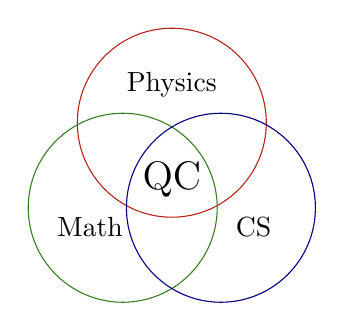
\begin{tikzpicture}[scale=0.6]
%  \begin{scope}
    \draw[color=BrickRed]   ( 90:1.2) circle (2);
    \draw[color=OliveGreen] (210:1.2) circle (2);
    \draw[color=NavyBlue]  (330:1.2) circle (2);
%  \end{scope}
  \node<1-> at ( 90:2)    {Physics};
  \node<2-> at ( 210:2)   {Math};
  \node<3-> at ( 330:2)  {CS};
  \node<4-> [font=\Large] {QC};
\end{tikzpicture}
&
\begin{minipage}[b]{0.5\textwidth}
\begin{itemize}
    \item<1->{\textcolor<1>{BrickRed}{Physics is the study of the observable universe}}
    \item<2->{\textcolor<2>{OliveGreen}{Math is the study of logic and reasoning}}
    \item<3->{\textcolor<3>{NavyBlue}{Computer science solves problems using computation}}
\end{itemize}

\end{minipage}
\end{tabular}
\only<4>{

\bigskip

Quantum Computing combines all of these disciplines}
\only<1>{\textcolor{BrickRed}{We study physics so as to understand and believe in quantum behavior}}
\only<2>{\textcolor{OliveGreen}{Quantum values and gates can be represented using linear algebra}}
\only<3>{\textcolor{NavyBlue}{Computer science lets us reason about the problems we can solve}}
\end{frame}

\begin{frame}{Goals}
\begin{itemize}
    \item 
\end{itemize}
\end{frame}